\section{Design}

The idea is really simple.
Hill climbing may include repetitive photo capturing and the minimum step of focus adjustment is too small which could be unnecessary.
To jump over this kind of duplication, we present \sysname, which picks a relatively large step of focus adjustment and collect all the photos needed in advance.
This method needs some additional space but can greatly save the repetitive work from hill climbing and suffers little photo quality penalty.

\begin{figure}[tb!]
	\begin{center}
		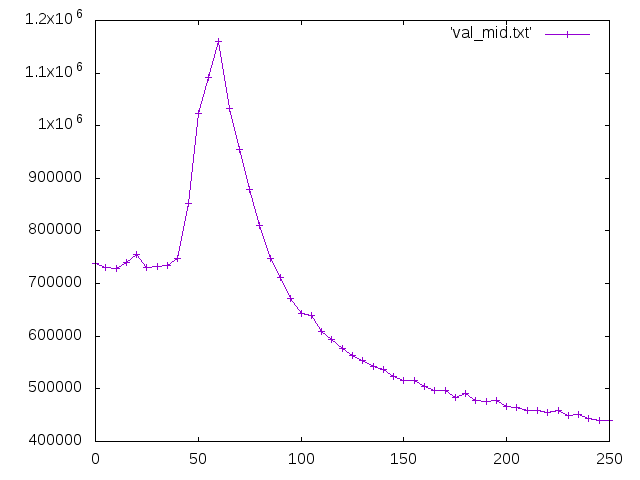
\includegraphics[width=2in]{midplot}
	\end{center}
	\caption{Inefficient hill climbing}
	\label{f:midplot}
\end{figure}

To verify that hill climbing is not efficient, we pick one of the earlier groups of photos as an example.
The focus function values for different focus positions are shown in Figure~\ref{f:midplot}.
Let us go through this group of photos according to hill climbing method.
Here we list them in sequence with both the focus position and the focus function value.

Step of 50: 250(440698), 200(466670), 150(516504), 100(644100), 50(1022550), 0(738123, getting smaller, reverse)

Step of 10: 10(728320), 20(755560), 30(732839), 40(748476), 50(1022550), 60(1159197), 70(955419, getting smaller, reverse)

Step of 5: 65(1032810), 60(1159197), 55(1092617, getting smaller, 5 is minimum step, stop at 60)

We can see that the global optimum is at focus position 60.
However, at the step of 50, the value did not get smaller, so focus actually goes to 0 first then gradually upwards via 10, 20, ...
This shows that this is different from normal binary search, and this one more step results in 6 more photos captured and 6 more focus function calculated.
Remember that hill climbing does not have additional memory so every time the value needs to be recalculated over and over again.

Just imagine, if we do the experiment under Windows where minimum step of 1 is supported, it could result in much much longer time of the focus process.

For \sysname, the details are shown below.
In Figure~\ref{f:param}, we can see that the focus position ranges from 0 to 250 and the minimum step is 5.
There are 2 versions of \sysname, where v1 has the step of 25 and v2 has the step of 50.
In other words, v1 takes photos only at the focus position of 0, 25, 50, 75, 100, 125, 150, 175, 200, 225 and 250, which includes 11 photos.
Similarly, v2 takes photos only at the focus position of 0, 50, 100, 150, 200, 250.

To evaluate our method, we also implement our version of hill climbing.
We implement hill climbing with the initial step of 50, then drops to 10 and finally to 5.
The initial position of focus is 250, which is the closest position from the camera sensor and has the clearest view of close objects.
When the process starts, it moves towards 0 and then switch when the focus function gets smaller.

To make the time of photo capturing more accurate, we take the photos at all focus positions (every 5 millimeters) in advance so that we can ignore the hardware time difference caused by the whole system.

We first tried ffmpeg as the photo capturing tool, but the time the process takes is just too long.
Taking one shot is over 1.5 seconds and that is not reasonable.
Now we use VideoCapture library in Python and it works perfectly.

The Laplacian operator is applied to every pixel of the photos and we use Python library as the implementation.
This could lead to slower process but as long as we use the same focus function implementation in the both hill climbing and \sysname, the results are still convincing.
